\documentclass[tikz,border=4pt]{standalone}

% Pure TikZ — compatible with minimal TinyTeX (pdflatex).
\usetikzlibrary{arrows.meta, positioning, calc, patterns,
                decorations.pathmorphing}

% -- B&W-safe palette --------------------------------------------------
\definecolor{steel}{HTML}{1a1a1a}
\definecolor{greyFill}{HTML}{c8c8c8}
\definecolor{sandFill}{HTML}{ece6d4}
\definecolor{scourFill}{HTML}{f5efe1}

% Geometry (prototype, m)
\def\D{2.0}       % bucket diameter (2R = 8 m prototype drawn as 2 cm)
\def\R{1.0}       % bucket radius
\def\L{2.3}       % skirt length = 9.3 m prototype
\def\Lbury{0.8}   % lid burial depth below mudline (arbitrary for clarity)

\def\S{0.9}       % example scour depth

\begin{document}
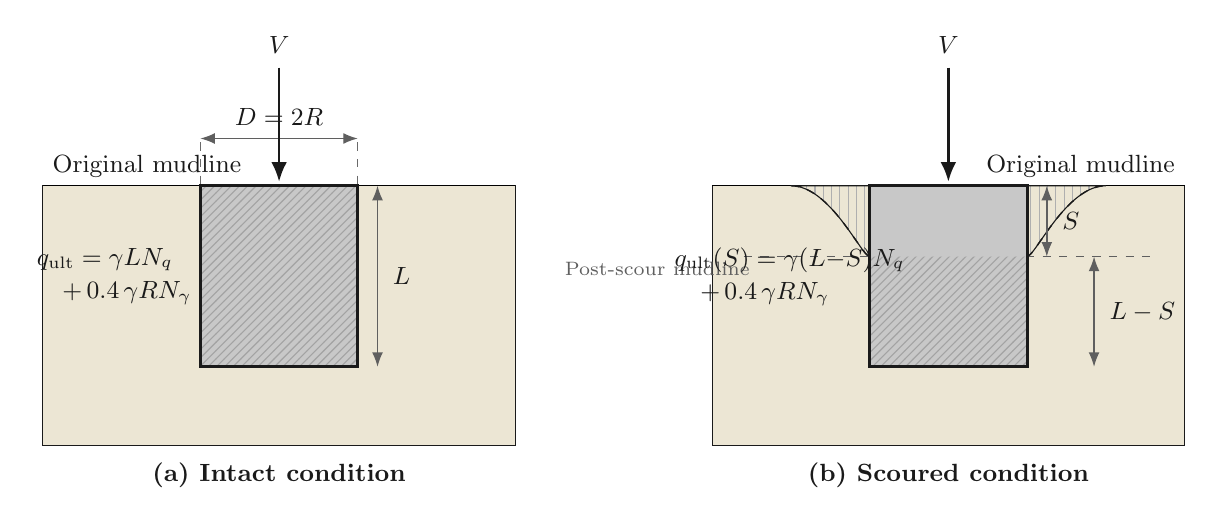
\begin{tikzpicture}[
    font=\sffamily\small,
    every node/.style={font=\sffamily\footnotesize},
    soil/.style={draw=steel, line width=0.4pt, fill=sandFill,
                 pattern color=steel!25},
    scour/.style={draw=steel, line width=0.4pt, fill=scourFill},
    bucket/.style={draw=steel, line width=1.0pt, fill=greyFill},
    dim/.style={Latex-Latex, line width=0.5pt, draw=steel!70},
    ldim/.style={-Latex, line width=0.5pt, draw=steel!85},
    nf/.style={-{Latex[length=2.5mm,width=2mm]}, line width=1.0pt,
               color=steel},
    label/.style={font=\small, color=steel},
    ]

% ====================================================================
% Panel (a) — Intact condition
% ====================================================================
\begin{scope}[local bounding box=panelA]

\def\ox{0}
\def\oy{0}

% Soil body
\fill[soil] (\ox-3,\oy-\L-1.0) rectangle (\ox+3,\oy);
\draw[line width=0.5pt] (\ox-3,\oy) -- (\ox+3,\oy);
\node[label, anchor=west] at (\ox-3,\oy+0.25) {Original mudline};

% Bucket geometry: lid at y=0, skirt extends to y=-L.
\fill[bucket] (\ox-\R,\oy-\L) rectangle (\ox+\R,\oy);
% Lid highlight
\draw[line width=1.2pt, color=steel] (\ox-\R,\oy) -- (\ox+\R,\oy);
% Hatched effective-capacity zone: full skirt length (intact)
\fill[pattern=north east lines, pattern color=steel!40]
  (\ox-\R,\oy-\L) rectangle (\ox+\R,\oy);
\draw[line width=1.0pt, color=steel]
  (\ox-\R,\oy-\L) rectangle (\ox+\R,\oy);

% Dimensions
\draw[dim] (\ox+\R+0.25,\oy) -- (\ox+\R+0.25,\oy-\L)
  node[midway, right=2pt, label]{$L$};
\draw[dim] (\ox-\R,\oy+0.6) -- (\ox+\R,\oy+0.6)
  node[midway, above=1pt, label]{$D = 2R$};
\draw[line width=0.4pt, color=steel!65, dashed]
  (\ox-\R,\oy+0.55) -- (\ox-\R,\oy);
\draw[line width=0.4pt, color=steel!65, dashed]
  (\ox+\R,\oy+0.55) -- (\ox+\R,\oy);

% Vertical load V at lid (single thick down-arrow)
\draw[nf] (\ox,\oy+1.5) -- (\ox,\oy+0.05);
\node[label, above] at (\ox,\oy+1.55) {$V$};

% N_q, N_gamma annotation
\node[label, align=left, anchor=west]
  at (\ox-\R-2.2,\oy-\L/2)
  {$q_{\mathrm{ult}} = \gamma L N_{q}$\\[1pt]$\quad+\,0.4\,\gamma R N_{\gamma}$};

% Panel title
\node[font=\bfseries\small, color=steel, anchor=north]
  at (\ox,\oy-\L-1.1) {(a) Intact condition};

\end{scope}

% ====================================================================
% Panel (b) — Scoured condition
% ====================================================================
\begin{scope}[local bounding box=panelB, shift={(8.5,0)}]

\def\ox{0}
\def\oy{0}

% Soil body (broader floor; scour bowl drawn as a void in the soil)
\fill[soil] (\ox-3,\oy-\L-1.0) rectangle (\ox+3,\oy);
\draw[line width=0.5pt] (\ox-3,\oy) -- (\ox+3,\oy);
\node[label, anchor=east] at (\ox+3,\oy+0.25) {Original mudline};

% Scour bowl around the bucket — depth = S
\fill[scour, pattern=vertical lines, pattern color=steel!35]
  (\ox-2.0,\oy) .. controls (\ox-1.5,\oy) and (\ox-\R-0.1,\oy-\S)
  .. (\ox-\R,\oy-\S)
  -- (\ox+\R,\oy-\S)
  .. controls (\ox+\R+0.1,\oy-\S) and (\ox+1.5,\oy)
  .. (\ox+2.0,\oy)
  -- cycle;
\draw[dashed, line width=0.5pt, color=steel]
  (\ox-2.0,\oy) .. controls (\ox-1.5,\oy) and (\ox-\R-0.1,\oy-\S)
  .. (\ox-\R,\oy-\S) -- (\ox+\R,\oy-\S)
  .. controls (\ox+\R+0.1,\oy-\S) and (\ox+1.5,\oy)
  .. (\ox+2.0,\oy);

% New effective mudline at base of scour (level with bucket-tip-minus-scour)
\draw[line width=0.5pt, color=steel!70, dashed]
  (\ox-2.6,\oy-\S) -- (\ox+2.6,\oy-\S);
\node[font=\scriptsize, anchor=east, color=steel!70]
  at (\ox-2.4,\oy-\S-0.15) {Post-scour mudline};

% Bucket (unchanged geometry)
\fill[bucket] (\ox-\R,\oy-\L) rectangle (\ox+\R,\oy);
% Hatched EFFECTIVE capacity zone: only portion below new mudline
\fill[pattern=north east lines, pattern color=steel!40]
  (\ox-\R,\oy-\L) rectangle (\ox+\R,\oy-\S);
% Grey (unhatched) portion above new mudline — zone with lost support
\fill[greyFill, draw=none, opacity=0.6]
  (\ox-\R,\oy-\S) rectangle (\ox+\R,\oy);
\draw[line width=1.0pt, color=steel]
  (\ox-\R,\oy-\L) rectangle (\ox+\R,\oy);

% Dimensions
\draw[dim] (\ox+\R+0.25,\oy) -- (\ox+\R+0.25,\oy-\S)
  node[midway, right=2pt, label]{$S$};
\draw[dim] (\ox+\R+0.85,\oy-\S) -- (\ox+\R+0.85,\oy-\L)
  node[midway, right=2pt, label]{$L-S$};

% Vertical load V at lid
\draw[nf] (\ox,\oy+1.5) -- (\ox,\oy+0.05);
\node[label, above] at (\ox,\oy+1.55) {$V$};

% Updated capacity formula
\node[label, align=left, anchor=west]
  at (\ox-\R-2.6,\oy-\L/2)
  {$q_{\mathrm{ult}}(S) = \gamma (L{-}S) N_{q}$\\[1pt]$\quad+\,0.4\,\gamma R N_{\gamma}$};

% Panel title
\node[font=\bfseries\small, color=steel, anchor=north]
  at (\ox,\oy-\L-1.1) {(b) Scoured condition};

\end{scope}

\end{tikzpicture}
\end{document}
